\documentclass[a4paper]{article}
\usepackage[utf8]{inputenc}
\usepackage[spanish, es-tabla, es-noshorthands]{babel}
\usepackage[table,xcdraw]{xcolor}
\usepackage[a4paper, footnotesep = 1cm, width=20cm, top=2.5cm, height=25cm, textwidth=18cm, textheight=25cm]{geometry}
%\geometry{showframe}

\usepackage{tikz}
\usepackage{amsmath}
\usepackage{amsfonts}
\usepackage{amssymb}
\usepackage{float}
\usepackage{graphicx}
\usepackage{caption}
\usepackage{subcaption}
\usepackage{multicol}
\usepackage{multirow}
\setlength{\doublerulesep}{\arrayrulewidth}
\usepackage{booktabs}

\usepackage{hyperref}
\hypersetup{
    colorlinks=true,
    linkcolor=blue,
    filecolor=magenta,      
    urlcolor=blue,
    citecolor=blue,    
}

\newcommand{\quotes}[1]{``#1''}
\usepackage{array}
\newcolumntype{C}[1]{>{\centering\let\newline\\\arraybackslash\hspace{0pt}}m{#1}}
\usepackage[american]{circuitikz}
\usetikzlibrary{calc}
\usepackage{fancyhdr}
\usepackage{units} 

\graphicspath{{../Ejercicio-1/}{../Ejercicio-2/}{../Ejercicio-3/}{../Ejercicio-4/}}

\pagestyle{fancy}
\fancyhf{}
\lhead{22.01 Teoría de Circuitos}
\rhead{Mechoulam, Lambertucci, Rodriguez Turco, Londero, Galdeman}
\rfoot{\centering \thepage}

\begin{document}
\subsection{Análisis Cualitativo del Circuito Base}

El siguiente análisis no cuantitativo del circuito base se comprobará más adelante a la hora de realizar las simulaciones y el subsiguiente prototipeado.

\subsubsection{Etapa de Alimentación}

La alimentación del circuito es una fuente no partida de $9V$. Se observa que el capacitor electrolítico $C_5$ se encuentra justo a la salida de la fuente de alimentación. Se presume que la utilidad de este es para filtrar cualquier ruido que haya montado sobre la continua, ya que por su conexión a tierra, cualquier tensión no contante encontrará un camino de baja impedancia hacia masa.

\begin{figure}[H]
	\centering
	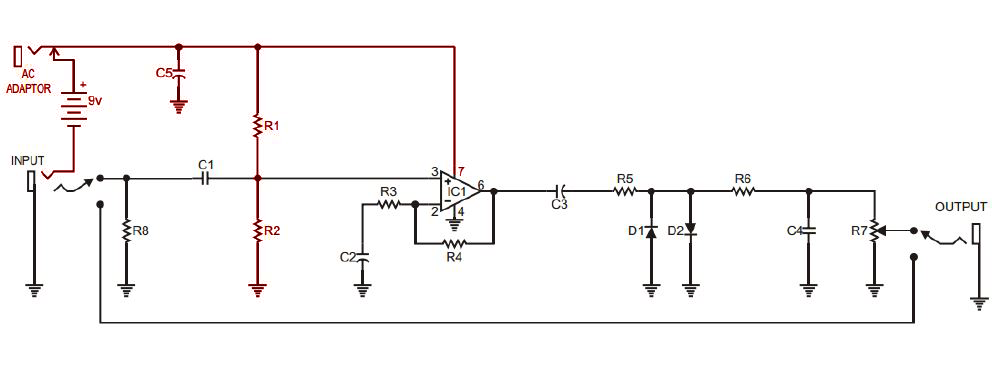
\includegraphics[width=1\textwidth, trim={0 0 0 0}, clip]{Ejercicio5/Imagenes/circuito_base_alimentacion.png}
	\caption{Alimentación del circuito base.}
	\label{fig:circuito_base_alimentacion}
\end{figure}

Luego pueden verse dos resistencias $R_1$ y $R_2$, donde $R_1$ está conectada a la señal de entrada y $R_2$ está conectada a la resistencia anterior y a tierra. Este par puede considerarse de manera aproximada como un divisor resistivo, ya que en el punto medio se ofrece gran impedancia por parte tanto del op-amp (despreciando la corriente de entrada) como por el capacitor $C_1$, ya que la tensión de alimentación es constante.
Este divisor resistivo lo que está haciendo es montando a la señal de entrada sobre la tensión en el punto medio. Es en este punto donde se soluciona el problema de tener una sola fuente no partida ya que, si se cumple que $R_1=R_2$, la señal de entrada quedará levantada $4.5V$, por lo que se podría alimentar al op-amp solo de manera positiva, llevando a tierra la alimentación negativa.\\

Por último, se llevan los $9V$ de la fuente de alimentación a la entrada de alimentación positiva del op-amp.


\subsubsection{Etapa de Pre-amplificación}

\begin{figure}[H]
	\centering
	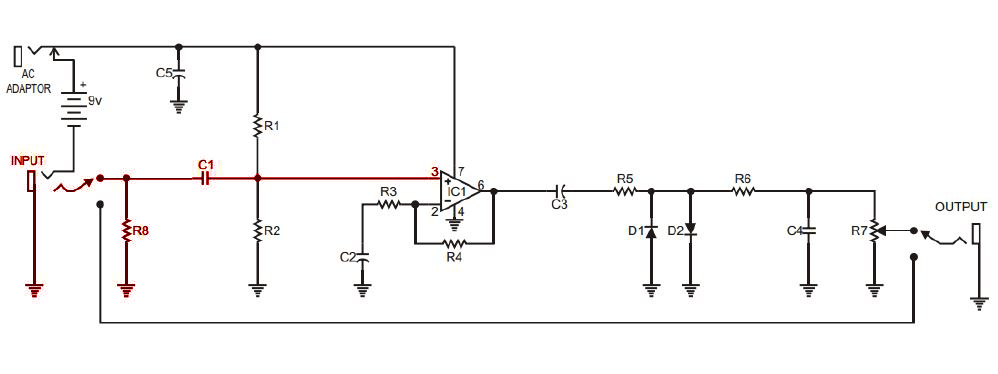
\includegraphics[width=1\textwidth, trim={0 0 0 0}, clip]{Ejercicio5/Imagenes/circuito_base_preamplificacion.png}
	\caption{Etapa de pre-amplificación del circuito base.}
	\label{fig:circuito_base_preamplificacion}
\end{figure}

Justo luego de la entrada se encuentra la resistencia $R_8$. Esta resistencia podría situarse en este lugar para atenuar levemente la entrada y ayudar a filtrar pequeños picos muy rápidos de tensión en la entrada. Otra hipótesis es que ayuda a elevar la impedancia de entrada de todo el circuito.\\

El capacitor $C_1$, como ya dicho antes, ofrece gran impedancia a la tensión continua de la alimentación para proteger a la entrada. De otra manera, la señal continua ingresaría por la entrada.
Lo que se obtiene posterior al capacitor será la señal de entrada levantada tantos voltios como proporcionen el punto medio del divisor resistivo.\\

Se contempla además que el circuito base nos permite tener una opción de realizar un bypass total al circuito mediante el uso de una llave de 

\subsubsection{Etapa de Amplificación}

El operacional se encuentra realimentado negativamente con una configuración no inversora. No es un problema que no este alimentado negativamente, ya que la señal de entrada estará montada sobre una continua.

\begin{figure}[H]
	\centering
	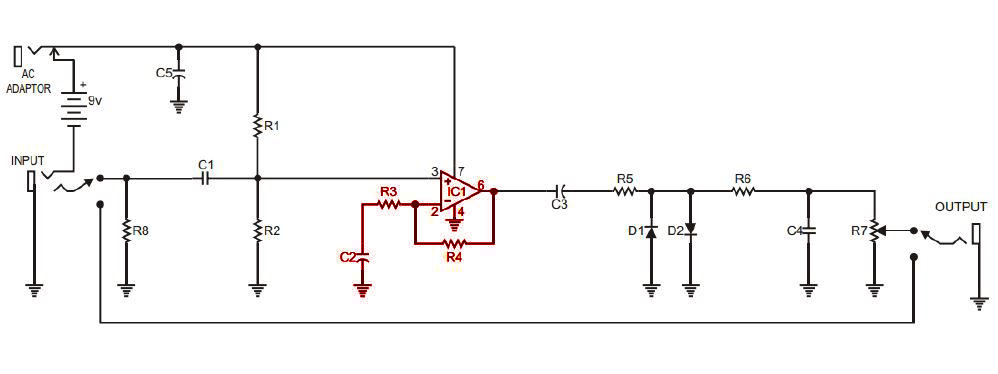
\includegraphics[width=1\textwidth, trim={0 0 0 0}, clip]{Ejercicio5/Imagenes/circuito_base_amplificacion.png}
	\caption{Etapa de amplificación del circuito base.}
	\label{fig:circuito_base_amplificacion}
\end{figure}

Analizando el lazo del op-amp, se puede observar que la realimentación dependerá de la frecuencia. Se realiza la hipótesis de que la transferencia actuará como un cero con una cierta frecuencia de corte. Esto también puede observarse ya que para bajas frecuencias el capacitor actúa como un circuito abierto, por lo que el op-amp se comportaría como un seguidor de tensión, ya que este intenta copiar la tensión de referencia en el pin numero 3. Para las frecuencias altas el operacional amplificará cada vez más la señal hasta llegar al polo dominante. Se observa como es aquí, en el lazo de realimentación, donde se podría controlar la amplificacion de las distintas frecuencias por separado.

\subsubsection{Etapa de Ecualización}

A la salida del operacional se encuentra el capacitor $C_3$. Este capacitor se utiliza para remover la continua sobre la cual estaba montada la señal de entrada.

\begin{figure}[H]
	\centering
	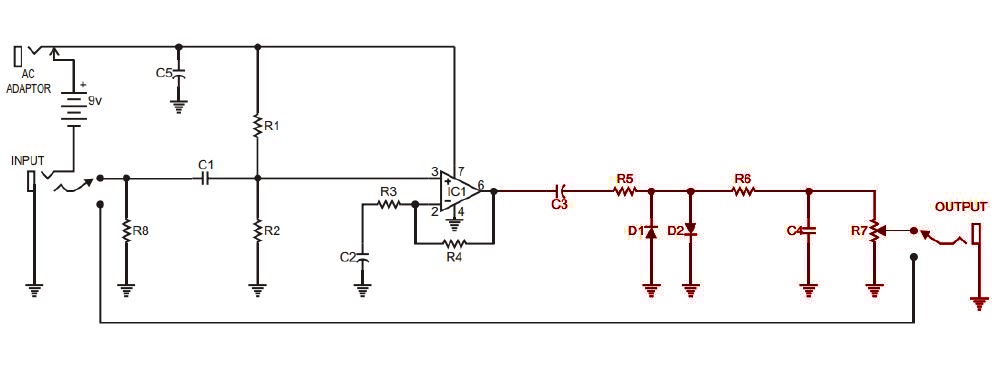
\includegraphics[width=1\textwidth, trim={0 0 0 0}, clip]{Ejercicio5/Imagenes/circuito_base_ecualizacion.png}
	\caption{Etapa de ecualización del circuito base.}
	\label{fig:circuito_base_ecualizacion}
\end{figure}

Luego, se encuentran en el circuito una resistencia en serie con un par de diodos en paralelo con polaridad invertida. Estos diodos fijarían la tensión de la señal en $V_{d_{on}}$ tanto para el semi-ciclo positivo como para el negativo. Esto deformaría a la señal generando un efecto de "clipping". Se presume que esto se apreciaría como una gran distorsión a la hora de conectar una guitarra y escuchar la salida.\\

Seguido de los diodos se puede encontrar un pequeño circuito R-C cuya finalidad podría ser la de darle un último cambio a la señal. Este circuito estaría atenuando las frecuencias altas. Se deberá comprobar mediante simulaciones y protobordeado el uso de este último tramo.

Finalmente antes de la salida se encuentra un potenciómetro, el cual se presume que se utiliza como control de volumen de salida.

\subsection{Análisis Cuantitativo del Circuito Base}

\large{ver R8 para que está si es que es solo impedancia de entrada}



 
\end{document}